\section{\texorpdfstring{Selection cuts for \Tau\Tau channel}{Selection cuts for tau-tau channel}}
\label{sect:tauTauCuts}
The selection of the events from the collisions for \Tau\Tau channel
is done with a dedicated trigger that uses the combination of 
two $\tau$ leptons reconstructed in the trigger levels \cite{CMS:2013hoa,Chatrchyan:2012xi,Chatrchyan:2011nv}.
The events with two \Tau's with \PT $>$ 35 \GeV and $|\eta|<$2.1 which have a medium isolation are recorded. 

To select the events for \Tau\Tau channel, two reconstructed \Tau which are oppositlely charged are selected. Both \Tau's are asked to 
have \PT $>$ 45 \GeV and $|\eta| <$ 2.1 and pass the medium isolation criteria.
%$I_{\Tau}$ less than 1\GeV. 
In the case of more than one pair, the pair with the tightest isolation 
%that minimizes the sum of $I_{\Tau}$ 
is selected.
The events with extra electrons or muons (\PT $>$ 10 \GeV, $\eta <$ 2.4 and loose isolation criteria) 
are rejected to suppress %the contribution of the associatiated production of \Z with vector bosons.
the background caused by diboson production.
%A Monte Carlo (MC) study shows that the invariant mass distribution of the two \Tau's coming from a \Z boson can be approximated 
%with a gaussian distribution with a peak close to 70 \GeV and a width of about 15 \GeV, so the events with the invariant mass of  
%the two \Tau's in this range are excluded (\Z-veto). 

The di-\Tau events that thier invariant mass is between 55 and 85 \GeV are rejected to suppress the \Z$\rightarrow$\Tau\Tau events (\Z veto).
A minimum cut of 15 \GeV on this invariant mass helps to get rid of the low mass
QCD resonances. The minimum angle in the transverse plane between the \MET and the jets with \PT $>$ 40 \GeV and $|\eta| <$ 5 
is asked to be greater than 1. This is a cut against the events with a fake \MET including the QCD multijet events. A soft cut on 
\mttwo ($>$ 40 \GeV) increases this rejection power.

After applying pre-selection cuts, two extra set of cuts are introduced which define the serach regions.
The first search region aims the points with large and medium mass difference between charginos and neutralinos, In this case,  \mttwo  distribution has a tail beyond the 
SM backgrounds. 
The other one is dedicated for low mass differences where sum of the \mt of two \Tau, \SumMT = $\mt^{\Tau^1} + \mt^{\Tau^2}$, can be a good descriminator between the signal and SM backgrounds.
The two signal regions are chosen to be exclusive in order 
to be able to combine the statistics at the end. 
%When the mass difference is sufficiently high, \mttwo has a tail well beyond 80 \GeV, which is 
%the peak  and the end point of the \mt distribution of $W$jets events in the parton level. 
%Due to the particles' width and the detector effects, 
%the endpoint is moved to the higher values and the optimized cut for this variable is 90 \GeV. 

%If the mass diffrenece is not too high, %\mttwo can not exceed 80 \GeV, but 
%the sum of the \mt of two \Tau, \SumMT = $\mt^{\Tau^1} + \mt^{\Tau^2}$, can be a good descriminator between the signal and SM backgrounds. 
Two signal regions are defined as:
\begin{itemize}
\item {\bf\binone}: \mttwo $>$ 90 \GeV;
\item {\bf\bintwo}: \mttwo $<$ 90 \GeV and \SumMT $>$ 250 \GeV; b-tagged jets are vetoed.
\end{itemize}
Vetoing the b-tagged jets in the second region is useful against the backgrounds containting a top quark, especially \ttbar events. 
To tag the b-jets, the medium working point of combined secondary vertex algorithm is used \cite{Chatrchyan:2012jua}. The b-jets have
\PT $>$ 20 \GeV and $|\eta| < $ 2.4.

The event yields can be found in table~\ref{tbl:cutflowtable}. The yields for three SUSY signal points, 
corresponding to a low mass difference $(m_{\chione}=180\GeV,~m_{\PSGczDo}=60\GeV)$, 
a moderate mass difference $(m_{\chione}=240\GeV,~m_{\PSGczDo}=40\GeV)$ and a high mass difference $(m_{\chione}=380\GeV,~m_{\PSGczDo}=1\GeV)$, are presented in the table.   
%\begin{sidewaystable}
\begin{table}[!Hhtb]
\begin{center}
\begin{small}
\begin{tabular}{lcccccccccc}
\hline\hline
  &SUSY(180,60)&(240,40)&(380,1)&Higgs&QCD&WW&W&DY&Top&Total Bkg\\%&Data\\
\hline\hline
%\multirow{5}{*}{Pre-Selection}&2 $\tau_h$ Selection&41.97&30.96&11.28&87.67&22081.57&13.71&595.80&2133.23&115.33&25027.32$\pm$6971.15&19615\\
%&$e$ and $\mu$ Veto&38.68&27.89&9.87&81.53&19272.05&11.21&543.42&1961.29&95.85&21965.34$\pm$6387.87&18526\\
%&Z Veo&37.80&26.28&9.21&70.50&18825.02&10.86&527.83&1333.37&88.53&20856.11$\pm$6383.93&17554\\
%&$\mindphifour > $ 1&17.95&15.16&6.13&13.91&8426.98&3.66&192.11&276.27&13.67&8926.59$\pm$4404.31&5105\\
%&$M_{T2} > $ 40&9.50&11.66&5.60&0.89&135.29&1.11&31.93&13.17&5.26&187.65$\pm$135.47&131\\
%\hline
%\binone&$M_{T2} > $ 90&0.59&3.89&3.81&0.17&$<$135.29&0.02&$<$1.28&0.56&$<$0.47&0.75$\pm$0.08&1\\
\binone &0.59&3.89&3.81&0.17& 0.0 &0.02&0.0&0.56&0.0 &0.75$\pm$0.08\\%&1\\
\hline
%\multirow{3}{*}{\bintwo}&b-jet veto&7.92 &9.33 &4.67 &0.75&135.20&0.96&29.13&11.15&0.78&177.98$\pm$135.36&115\\
%&$M_{T2} < $ 90&7.42 &6.17 &1.51 &0.61&135.20&0.94&29.13&10.65&0.78&177.32$\pm$135.36&114\\
\bintwo &2.17&3.36  &1.08&0.07& 0.0 &0.15&0.43&0.81&0.53&1.99$\pm$0.87\\%&2\\
\hline\hline
\end{tabular}
\caption{ MC driven yields for $\tauTau$ channel. The quoted uncertainties are only statistical.}
\label{tbl:cutflowtable}
\end{small}
\end{center}
\end{table}
%\end{sidewaystable}

The distributions of $\mttwo$ and $\SumMT$ after applying these pre-selection cuts are shown in figure~\ref{fig:comparison}.
The b-jet veto cut is also applied on the $\SumMT$ distribution. For both plots, the shape of QCD multijet events
is taken from same-sign data events, which means that same selection cuts as pre-selection are applied except for the charge
requirement which is reversed. The same-sign data is dominated by QCD. The same-sign non-QCD MC is subtracted from the same-sign data to
find the distribution of QCD in opposite-sign region.   
 It can be concluded that data and MC are in reasonable agreement within the statistical uncertainties.
\begin{figure}[!Hhtb]
\centering
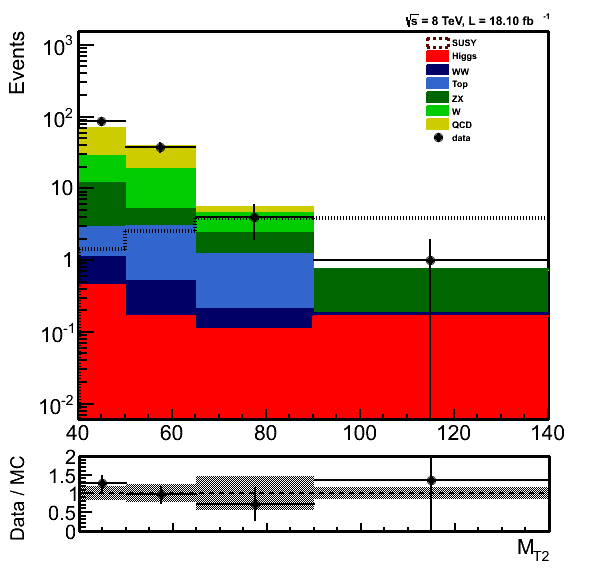
\includegraphics[angle=0,scale=0.35]{TauTauFigs/MT2_SSQCD_dataunblinding.png}
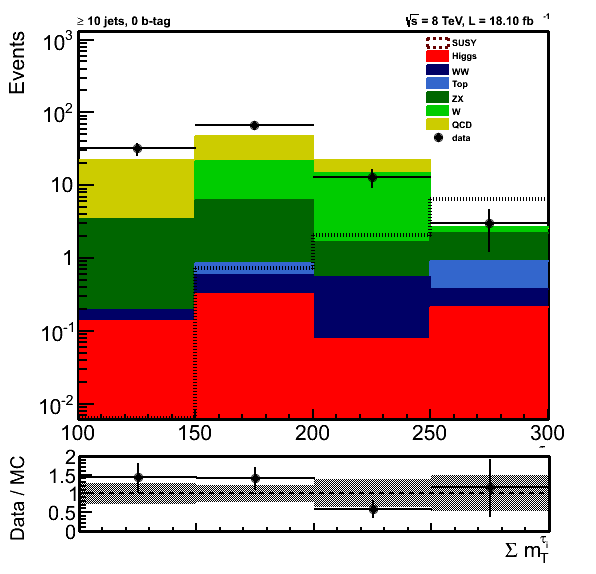
\includegraphics[angle=0,scale=0.35]{TauTauFigs/SumMT_SSQCD_dataunblinding.png} \\
\caption{The distributions of \mttwo (left) and \SumMT (right) after pre-selection. The b-jet veto cut is also applied on the right plot.}
\label{fig:comparison}
\end{figure}
